\chapter{Methods}

\section{Registration}
``Image registration is the process of overlaying two or more images
of the same scene taken at different times, from different viewpoints,
and/or by different sensors. It geometrically align two images --the
reference and sensed images.''\cite{zitova}

``Image registration is a crucial step in all image analysis tasks in
which the final information is gained from the combination of various
data sources like in image fusion, change detection, and multichannel
image restoration.''\cite{zitova}\\


The following images show a checkerboard comparison of two volumes
taken of the same patient at different times. Figure \ref{before_reg}
shows the image comparison before performing affine
registration. Figure \ref{after_reg} shows the comparison of images
after the registration has been done.

\begin{figure}[htb]
  \centering
  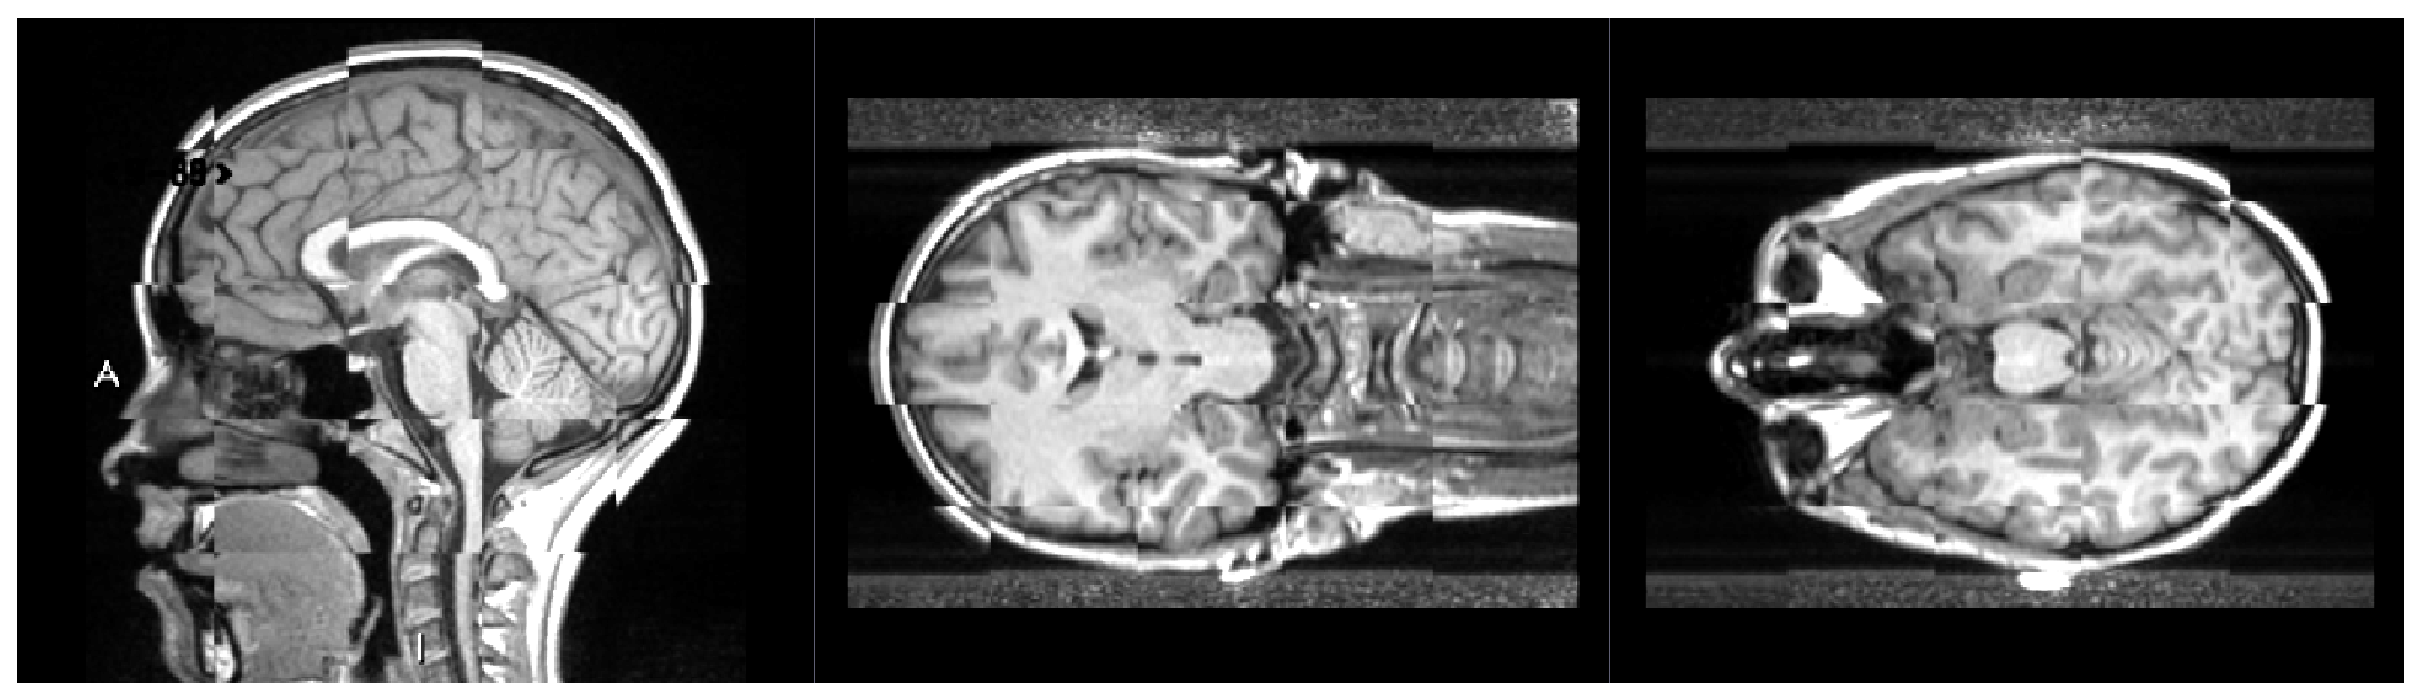
\includegraphics[scale=0.3]{before_registration.eps}
  \caption{Comparison of volumes before registration}
  \label{before_reg}
\end{figure}


\begin{figure}[htb]
  \centering
  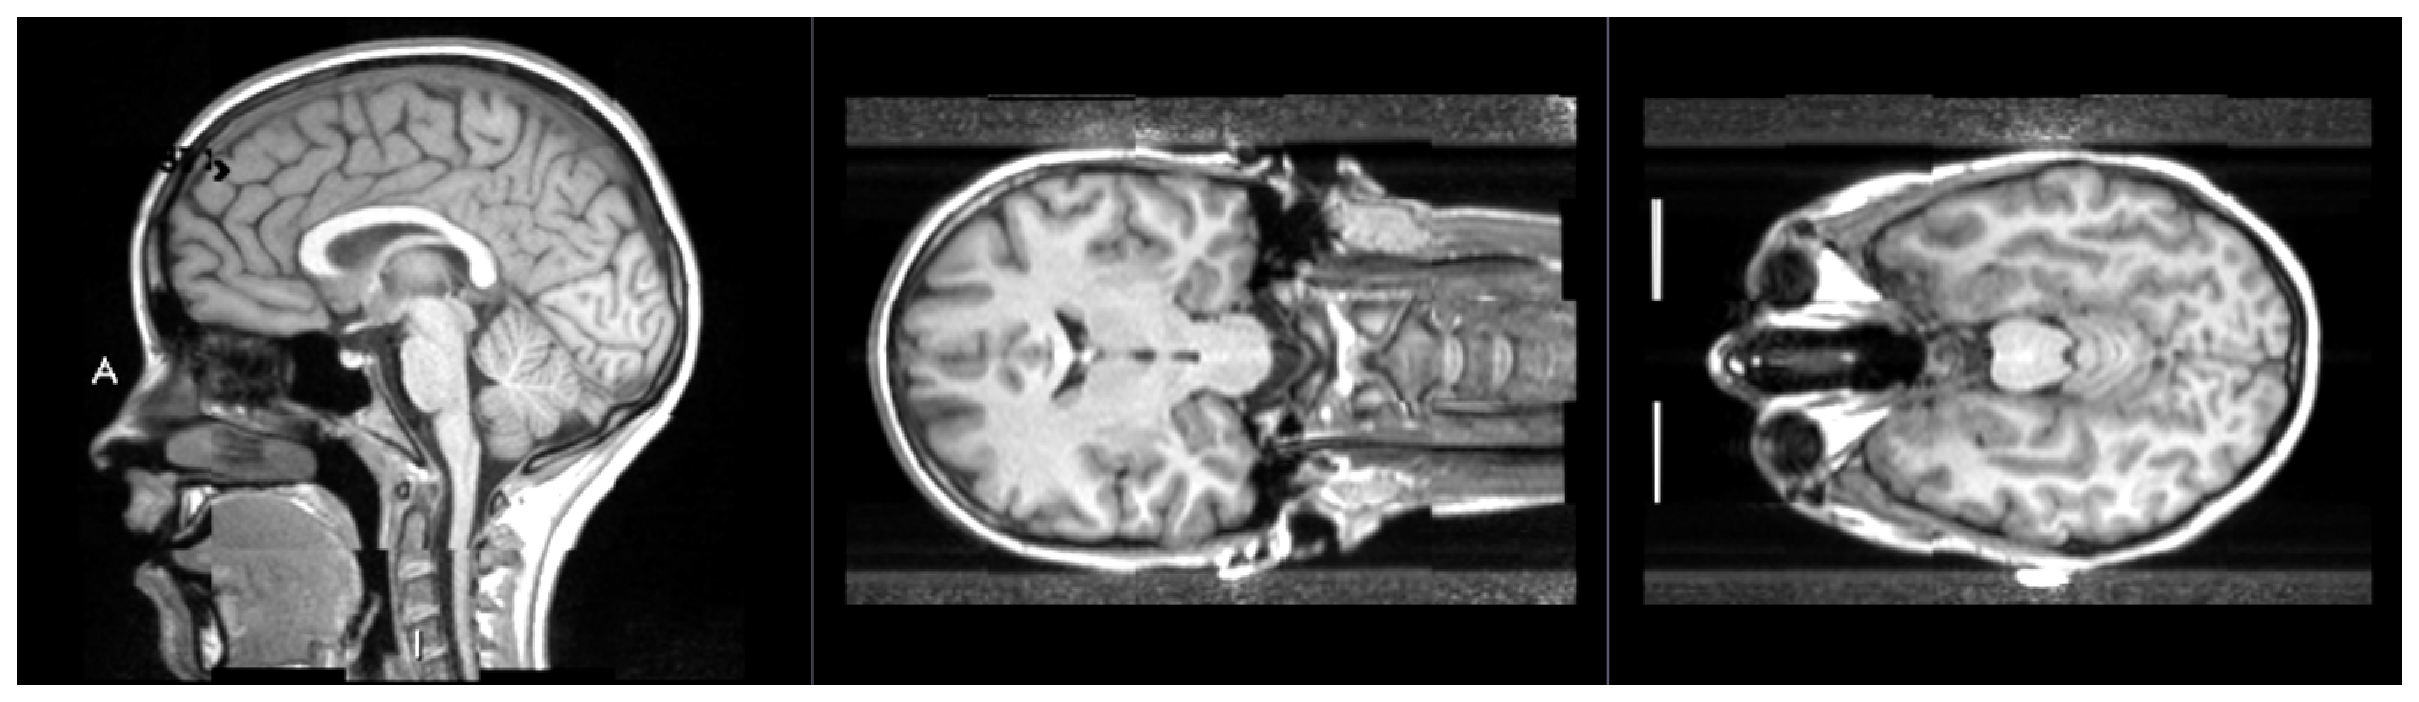
\includegraphics[scale=0.3]{after_registration.eps}
  \caption{Comparison of volumes after registration}
  \label{after_reg}
\end{figure}

The second volume has been modified using affine registration so that
the comparison between both volumes becomes much easier.\\

According to \cite{zitova}, the majority of the registration methods consist of the following steps:
\begin{enumerate}
\item \textit{Feature detection:} Salient and distinctive objects are detected.
\item \textit{Feature matching:} The correspondence between the features detected in the sensed image and those detected in the reference image is established.
\item \textit{Transform model estimation:} The type and parameters of the mapping functions are estimated. These functions align the sensed image with the reference image.
\item \textit{Image resampling and transformation:} The sensed image is transformed by means of the mapping functions.
\end{enumerate}


\subsection{Registration Methods used}
\label{sec:reg_methods}
There are many different methods to accomplish registration between
images or volumes. In this project only a few of these methods were
used based on experiments performed with some of the available
methods. The chosen procedures were the ones that behaved better
under the specific conditions of this work.


\subsubsection{Affine Registration}
In geometry, an \textit{affine transformation} or an \textit{affinity}
is a transformation which preserves straight lines (i.e., all points
lying on a line initially still lie on a line after the
transformation) and ratios of distances between points lying on a
straight line. It does not necessarily preserve angles or lengths, but
does have the property that sets of parallel lines will remain
parallel to each other after an affine transformation \cite{affine_t}. \\

The implementation of affine registration used during this project is
the one included in \textit{3D Slicer} version 4.1. 

The application is able to register two images together using an
affine transform and mutual information, and it allows the user to
modify quite a few parameters
in order to obtain the expected result.\\

If you would like to know more about this implementation of affine
registration please refer to the module webpage:

\url{http://wiki.slicer.org/slicerWiki/index.php/Documentation/4.1/Modules/AffineRegistration}

\subsubsection{B-Spline Registration}
In the mathematical subfield of numerical analysis, a
\textit{B-spline} is a spline function that has minimal support with
respect to a given degree, smoothness, and domain partition.

However, in computer graphics, the term \textit{B-spline} frequently
refers to a spline curve parametrized by spline functions that are
expressed as linear combinations of \textit{B-splines} (in the
mathematical sense explained above) \cite{bspline}.\\

Just like in the case of affine registration, the implementation of
B-Spline registration used during this project is the one included in
\textit{3D Slicer} version 4.1. 

The application divides the volumes into a grid of user-defined size
in which each line is a B-spline that will be modified by the
registration to create a transform that aligns the two volumes.\\

If you would like to know more about this implementation of B-spline
registration please refer to the module webpage:

\url{http://wiki.slicer.org/slicerWiki/index.php/Documentation/4.1/Modules/BSplineDeformableRegistration}


\subsubsection{BRAINS Demon Warp Registration}
As with the registration methods explained before, \textit{BRAINS
  Demon Warp} registration is implemented as a module in \textit{3D
  Slicer} version
4.1.\\

The module works by using the ITK filter based on Thirion's Demons
algorithm, in which the main idea is to consider the objects
boundaries in one image as semi-permeable membranes and to let the
other image, considered as a deformable grid model, diffuse through
these interfaces, by the action of effectors situated within the
membranes. \cite{thirion}.

An important characteristic of this implementation, that was
particularly useful for this project, is that it can produce a
\textit{deformation field} as the output of the registration. A
deformation field is a vector image in which each point is a vector
that indicates the amount of deformation necessary
at that point in order to align the volumes.\\


If you would like to know more about the implementation of
\textit{BRAINS Demon Warp} registration please refer to the module
webpage:

\url{http://wiki.slicer.org/slicerWiki/index.php/Documentation/4.1/Modules/BRAINSDemonWarp}


\section{Morphometry}
Morphometry refers to the measurement of external form. More
specifically, \textit{brain morphometry} is concerned with the
measurement of brain structures and changes thereof during
development, aging, learning, disease and evolution. Its goal is to
derive specific information from noninvasive neuroimaging data of live
brains, typically obtained from magnetic resonance imaging (MRI); and
to quantify the anatomical features of the brain in terms of shape,
mass and volume \cite{brmorph}.\\

In general, brain morphometry can be divided into three different methods: \textit{deformation-based}, \textit{tensor-based} and \textit{voxel-based} morphometry. Defined briefly as:
\begin{itemize}
\item \textit{Deformation-based:} Uses deformation fields to identify differences in the relative positions of structures.
\item \textit{Tensor-based:} Uses deformation fields to identify differences in the local shape of brain structures.
\item \textit{Voxel-based:} Uses voxel-wise comparison of the local concentration of grey matter.
\end{itemize}


\subsection{Morphometry methods used}
\label{sec:morph_methods}
Only \textit{tensor-based} and \textit{voxel-based} morphometry
methods where used during this project, since their outputs were
easier to adapt to our requirements.


\subsubsection{Voxel-based Morphometry}
A useful measure of structural difference among populations is derived
from a comparison of the local composition of different brain tissue
types (e.g., grey matter, white matter, etc). Voxel-based morphometry
(VBM) has been designed to be sensitive to these differences, while
discounting positional and other large scale volumetric differences in
gross anatomy.

Since its inception, VBM has become an established tool in morphometry
being used to detect cortical atrophy and differences in slender white
matter tracts \cite{ashburner}.\\

An objection to VBM is that it is sensitive to systematic shape
differences attributable to misregistration. Many potential
differences can arise as a result of movement or different positioning
of the subject in the scanner, and also there can be systematic
differences in the relative intensity of grey matter voxels compared
to white matter \cite{ashburner}.

All these differences can be detected by VBM since they are all real
differences among the data, even when they may not imply an increase
or reduction in grey matter density.\\

When VBM is used to compare MRI data of many different subjects, as is
the case many times, the process involves spatially normalizing all
the images to the same stereotactic space, extracting the gray matter
from the normalized images, smoothing, and finally performing a
statistical analysis to localize, and make inferences about, group
differences. The output from the method is a statistical parametric
map showing regions where gray matter concentration differs
significantly between groups \cite{ashburner2}.\\


For a detailed step-by-step description of VBM, please refer to
\cite{ashburner2}.

\subsubsection{Tensor-based Morphometry}
The goal of tensor-based morphometry (TBM) is to determine regional
shape differences. 

A deformation field that maps one image to another can be considered a
discrete vector field. By taking the gradients at each element of the
field, a \textit{Jacobian matrix} field is obtained, in which each element is a
tensor describing the relative positions of the neighboring
elements. Morphometric measures derived from this tensor field can be
used to locate regions with different shapes. The field obtained by
taking the determinants at each point gives a map of the structure
volumes relative to those of a reference image \cite{ashburner2}.\\

In principle, the \textit{Jacobian matrices} of the deformations (a
2nd order tensor field relating to the spatial derivatives of the
transformation) should be more reliable indicators of brain shape than
absolute deformations. Absolute deformations represent positions of
brain structures, rather than local shape, and need to be quantified
relative to some arbitrary reference position \cite{ashburner}.\\

A \textit{Jacobian matrix} contains information about the local
stretching, shearing and rotation involved in the deformation, and is
defined at each point by:

\[
J = \begin{bmatrix}
  \frac{\partial y_1}{\partial x_1} & \frac{\partial y_1}{\partial x_2} & \frac{\partial y_1}{\partial x_3} \\[0.3em]
  \frac{\partial y_2}{\partial x_1} & \frac{\partial y_2}{\partial x_2} & \frac{\partial y_2}{\partial x_3} \\[0.3em]
  \frac{\partial y_3}{\partial x_1} & \frac{\partial y_3}{\partial x_2} & \frac{\partial y_3}{\partial x_3}
\end{bmatrix}
\]\\

The form of TBM that was used in this project involves comparing
relative volumes of different brain structures, where the volumes are
derived from \textit{Jacobian determinants} at each point. According
to \cite{ashburner}, this type of morphometry is useful for studies
that have specific questions about whether growth or volume loss has
occurred, and so is appropriate for our problem.\\

The \textit{Jacobian determinant} is the determinant of the
\textit{Jacobian matrix} and is sometimes simply called ``the
Jacobian''.

For a differentiable function $f$ (a function whose derivative exists
at each point in its domain), the \textit{Jacobian determinant} of
$f$'s \textit{Jacobian matrix} at a given point gives important
information about the behavior of $f$ near that point.

For instance, if the \textit{Jacobian determinant} at a point $p$ is
positive, then $f$ preserves orientation near $p$; if it is negative,
$f$ reverses orientation. The absolute value of the \textit{Jacobian
  determinant} at $p$ gives us the factor by which the function $f$
expands or shrinks volumes near $p$ \cite{jacobian}.




